\section{Comparison of the Predictions with the Measured Data}
\label{secDataMCcomparison}


A comparison of the background spectrum measured during the commissioning run in Fall 2009 (run07) and the Monte Carlo simulation is shown in Figure~\ref{figDataMC_FS} for the 30~kg fiducial volume without veto cut. The energy region below 100~keV is shown separately in Figure~\ref{figDataMC_WS}. 

\begin{figure}[!b]
\centering
%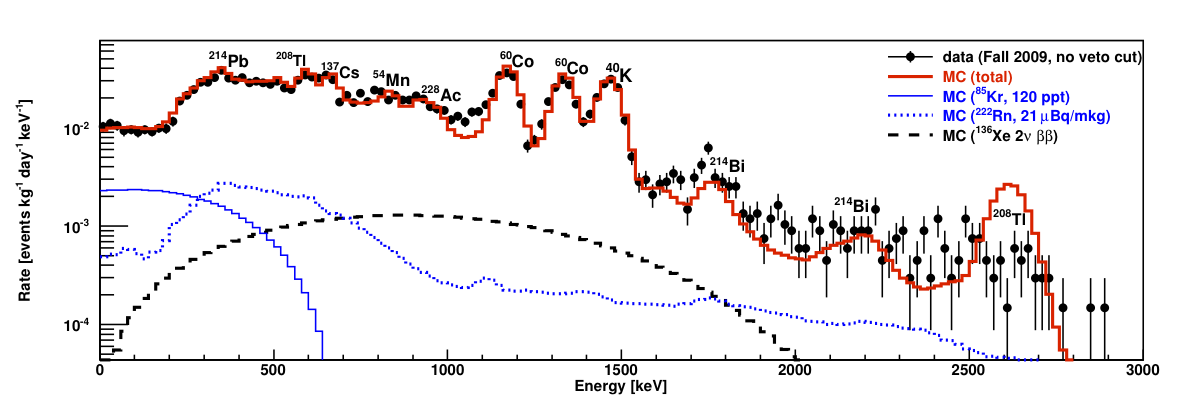
\includegraphics[width=1.0\linewidth]{plots/DataMC/dataMC_30kg_PassiveVeto_FS1.png}
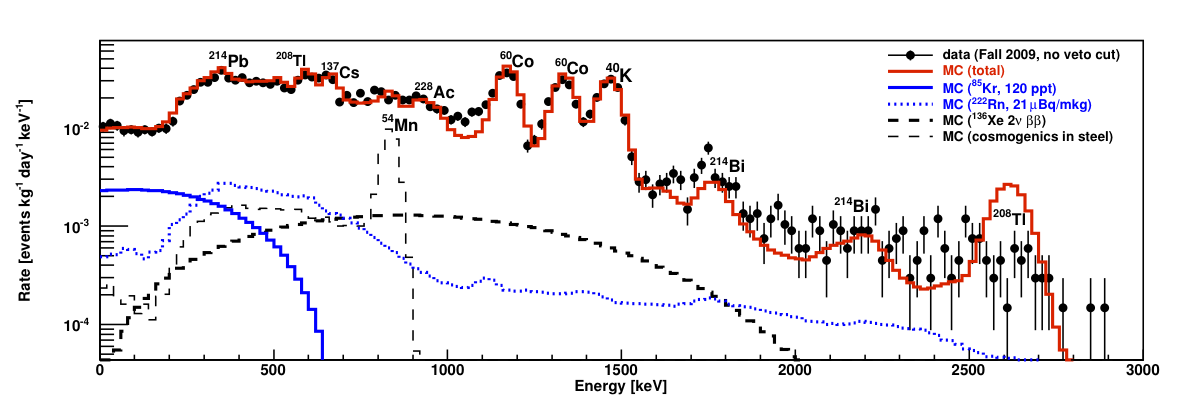
\includegraphics[width=1.0\linewidth]{plots/DataMC/dataMC_FS.png}
\caption[Background spectrum measured in the commissioning run in Fall 2009 and Monte Carlo simulations in the 30~kg fiducial volume without veto cut]{Background spectrum from measured data (commissioning run in Fall 2009~\cite{xe100-run07}) and from Monte Carlo simulations in the 30~kg fiducial volume without veto cut. Cosmogenic activation of LXe is not included. The energy spectra of $^{85}$Kr and  $^{222}$Rn decays in LXe are shown with the thin blue solid and dotted lines, respectively. The thin black dashed histogram shows the theoretical spectrum of the 2$\nu$ double beta decay of $^{136}$Xe, assuming a half-life of 1.1$\times$10$^{22}$~years~\cite{DoubleBetaLimit}. }
\label{figDataMC_FS}
\end{figure}

For optimal energy resolution and improved linearity, the energy scale of the measured spectrum exploits the anti-correlation between the light and the charge, as described in Section~\ref{secCES}. The definition of the combined energy scale has been adjusted on the $^{40}$K and $^{60}$Co peaks:
\begin{equation}
\label{eqCES_BG}
\mathrm{CES}_{\mathrm{BG}}\ \text{[keV]} = \mathrm{S}1_{\mathrm{total}} \cdot 0.227 + \mathrm{S}2_{\mathrm{bottom}} \cdot (7.545\times10^{-3}).
\end{equation}

The simulated spectrum is smeared with a Gaussian function using the energy resolution measured with calibration sources, following the functional dependence as in equation (\ref{eqResCES}).
% The contribution from the detector and shield materials is scaled based on the radioactive screening (Section~\ref).
For the level of $^{222}$Rn in the shield cavity, the upper limit measured with a dedicated radon monitor has been used. For the $^{222}$Rn level in the LXe, the value determined with the delayed coincidence analyses described in Section~\ref{secDelayedCoincidenceRn222} has been applied.

The level of $^{85}$Kr of 120~ppt has been inferred from the best fit of the simulated and measured spectra. For the first science run (run08), the krypton concentration inferred by this method is (700$\pm$100)~ppt. These results are in a good agreement with the delayed coincidence measurements described in Section~\ref{secDelayedCoincidenceKr85}. 

\begin{floatingfigure}[lh]{0.475\textwidth}
%\begin{figure}[!h]
\centering
%\subfigure[]{
%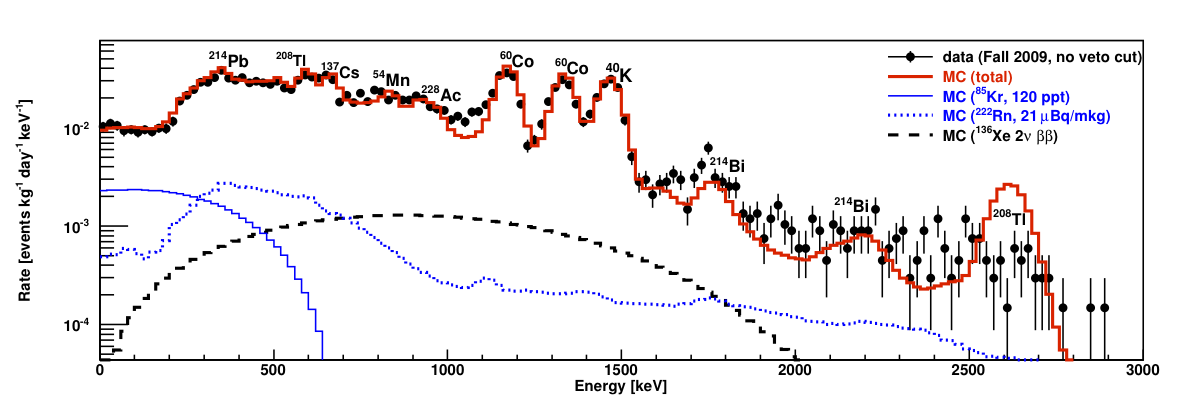
\includegraphics[width=0.475\linewidth]{plots/DataMC/dataMC_30kg_PassiveVeto_FS1.png}
%\label{figPMTtestSER_1}}
%\subfigure[]{
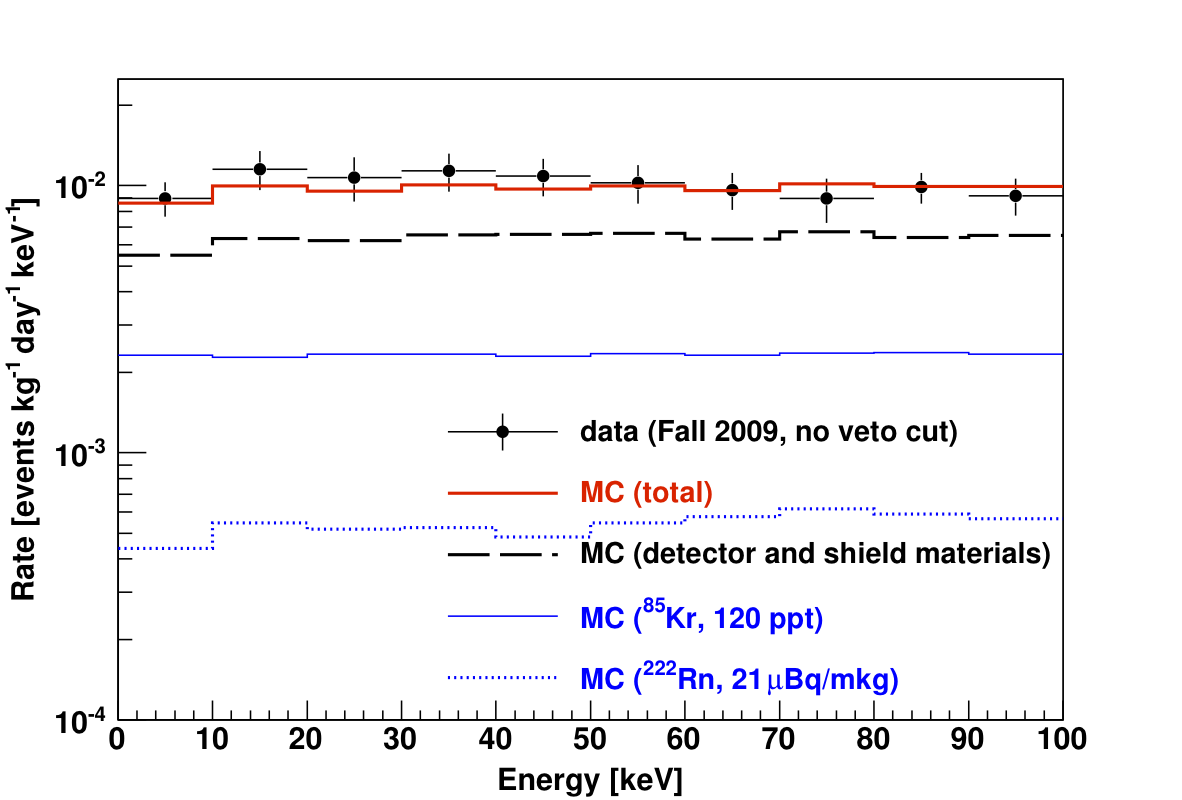
\includegraphics[width=0.475\linewidth]{plots/DataMC/dataMC_30kg_PassiveVeto_WS2.png}
%\label{figPMTtestSER_2}}
\caption[Low energy region of the measured and simulated background spectra]{Zoom into the low energy region of Figure~\ref{figDataMC_FS}: energy spectra of the measured background and Monte Carlo simulations in the 30~kg fiducial volume without veto cut. The  2$\nu~\beta\beta$ decay of $^{136}$Xe has negligible contribution to the background below 100~keV. Figure published in Ref.~\cite{EMBG}.}
\label{figDataMC_WS}
%\end{figure}
\end{floatingfigure}

Very good agreement of the background model with the data is achieved for the low energy region, below 700~keV, and for the main peaks: $^{214}$Pb (352~keV), $^{208}$Tl~(583 keV), $^{137}$Cs~(662 keV), $^{60}$Co (1173 and 1332~keV), and $^{40}$K (1460~keV). In particular, simulated and measured background spectra agree well in the energy region of interest, below 100~keV (Figure~\ref{figDataMC_WS}). The predicted rates of single scatter electronic recoil events in the energy region of interest are presented in Table~\ref{tabSummaryElectronRecoilsPassiveVeto}. In the 30~kg fiducial volume, $^{85}$Kr contributes $\sim$30\% to the total background without veto cut, and 55\% when a veto coincidence cut with an average energy threshold of 100~keV is applied. The contribution from $^{222}$Rn in the LXe is $<$7\%, from $^{222}$Rn in the shield cavity $<$2\% of the total background rate in the energy region of interest.

The disagreement between simulated and measured spectra above $\sim$1.5~MeV is caused by  non-linear effects in the PMT response, which result in a worse performance of the position reconstruction algorithms, as explained in Section~\ref{secPosRecSaturation}, changing the rate in the fiducial volumes and leading to a worsening of the position dependent signal corrections. 

Using only the measured radioactive contamination, the background model shows a deficit in the 700-1100~keV range. Most of this deficit can be explained by cosmogenic activation of the stainless steel parts during materials storage and detector construction, in particular the $^{54}$Mn isotope with a half-life of 312~days. The activity assumed in the present study is 1.25~mBq/kg, and the decays have been generated uniformly in all parts made of 316Ti SS. This value is within the limit calculated in Section~\ref{secCosmogenicActivationSteel} from the saturation activity measured for the activation at LNGS level. The predicted background from the cosmogenic activation in the stainless steel is at the level of 10$^{-4}$~events$\cdot$kg$^{-1}\cdot$day$^{-1}\cdot$keV$^{-1}$, thus about 5\% of that from natural radioactivity in the same components.

Cosmogenic activation of natural xenon, discussed in Section~\ref{secCosmogenicActivationLXe}, cannot explain the remaining discrepancy around 1100~keV without destroying the remarkable agreement in other energy ranges. 

The theoretical spectrum of the 2$\nu$ double beta decay of $^{136}$Xe is also shown in Figure~\ref{figDataMC_FS},  assuming the current half-life limit of 1.1$\times$10$^{22}$~years~\cite{DoubleBetaLimit}. Its contribution does not change the total background spectrum significantly, thus it can be concluded that the small remaining discrepancy between measured and simulated spectra can not be explained by this potential background source. The predicted energy averaged background rate from the 2$\nu~\beta\beta$ decay of $^{136}$Xe is at the level of 10$^{-6}$~events$\cdot$kg$^{-1}\cdot$day$^{-1}\cdot$keV$^{-1}$ below 100~keV, three orders of magnitude lower than the background from other components. 

The predicted rate of single scatter electronic recoil events in the energy region below 100~keV is shown in Tables~\ref{tabSummaryElectronRecoilsPassiveVeto} and \ref{tabSummaryElectronRecoilsActiveVeto}, without and with the veto coincidence cut, respectively. Discrimination between electron and nuclear recoils based on the ratio of proportional to primary scintillation light (S2/S1) is not considered here, and provides a further background reduction of~$>$99\%.

%The predicted rate of single scatter electronic recoil events in the energy region below 100~keV, without veto coincidence cut is 15.8$\times$10$^{-3}$ (9.6$\times$10$^{-3}$) events$\cdot$kg$^{-1}\cdot$day$^{-1}\cdot$keV$^{-1}$ for 40~kg (30~kg) fiducial mass (Table~\ref{tab:summaryElectronRecoils}). By applying a veto cut with an average energy threshold of 100~keV, these rates are reduced to 6.1$\times$10$^{-3}$ (4.6$\times$10$^{-3}$)~events$\cdot$kg$^{-1}\cdot$day$^{-1}\cdot$keV$^{-1}$ for 40~kg (30~kg) fiducial mass. 

Based on the values from Tables~\ref{tabSummaryElectronRecoilsPassiveVeto} and ~\ref{tabSummaryElectronRecoilsActiveVeto}, the contribution from various sources to the total background in the 30~kg fiducial volume has been calculated, and shown as pie-charts in Fig.~\ref{figPies}. The natural radioactivity in the detector and shield components dominates the total background (70\%), when the veto coincidence cut is not used. With the veto coincidence cut the background from external sources is reduced by a factor of $\sim$3, and $^{85}$Kr contamination in the liquid xenon contributes about 50\% to the total background.

\begin{table}[!h]
\centering
\caption[Summary of the predicted electronic recoil background without veto cut]{Summary of the predicted electronic recoil background: rate of single scatter events in the energy region below 100~keV, before S2/S1 discrimination and {\it without veto cut}.}
\label{tabSummaryElectronRecoilsPassiveVeto}
%\vspace{0.2cm}
\begin{tabular}{>{\footnotesize}l |>{\footnotesize} c |>{\footnotesize} c |>{\footnotesize} c |>{\footnotesize} c }
%\begin{tabular}{l | c | c | c | c }
\hline
&  \multicolumn{4}{>{\footnotesize}c}{[$\times$10$^{-3}$ events$\cdot$kg$^{-1}\cdot$day$^{-1}\cdot$keV$^{-1}$]}\\
\hline
Volume &  62~kg & 48~kg & 40~kg & 30~kg \\
\hline
%Veto cut & \multicolumn{1}{c|}{~~none~~} & \multicolumn{1}{c|}{active} & \multicolumn{1}{c|}{~~none~~} & \multicolumn{1}{c|}{active} & \multicolumn{1}{c|}{~~none~~} & \multicolumn{1}{c}{active} \\
Detector and shield materials			& 134.39 	& 17.23	& 11.93	  	& 6.54  	\\
$^{222}$Rn in the shield (1~Bq/m$^{3}$)	& 5.95 	& 1.13	& 0.92	  	& 0.16 	\\
$^{222}$Rn in LXe (21~$\mu$Bq/kg)	& 1.04   	& 0.63	& 0.56 	       	& 0.53  	\\
run07: $^{85}$Kr in LXe (120~ppt of $^{\mathrm{nat}}$Kr) 	& 2.35   	&  2.35	& 2.35 	 	& 2.35  	\\
run08: $^{85}$Kr in LXe (700~ppt of $^{\mathrm{nat}}$Kr) 	& 13.71   	&  13.71	& 13.71 	 	& 13.71  	\\
\hline
All sources, run07  					& 143.73	& 21.34 	& 15.76 	     	& 9.58  	\\
All sources, run08  					& 154.88	& 32.70 	&  27.12		& 20.94  	\\
\hline
\end{tabular}
\end{table}

\begin{table}[!h]
\centering
\caption[Summary of the predicted electronic recoil background with veto coincidence cut]{Summary of the predicted electronic recoil background: rate of single scatter events in the energy region below 100~keV, {\it with the veto coincidence cut} with an average energy threshold of 100~keV. The efficiency of electronic recoil discrimination based on S2/S1 ratio is not taken into account.}
\label{tabSummaryElectronRecoilsActiveVeto}
%\vspace{0.2cm}
\begin{tabular}{>{\footnotesize}l |>{\footnotesize} c |>{\footnotesize} c |>{\footnotesize} c |>{\footnotesize} c }
%\begin{tabular}{l | c | c | c | c }
\hline
&  \multicolumn{4}{>{\footnotesize}c}{[$\times$10$^{-3}$ events$\cdot$kg$^{-1}\cdot$day$^{-1}\cdot$keV$^{-1}$]}\\
\hline
Volume &  62~kg & 48~kg & 40~kg & 30~kg \\
\hline
%Veto cut & \multicolumn{1}{c|}{~~none~~} & \multicolumn{1}{c|}{active} & \multicolumn{1}{c|}{~~none~~} & \multicolumn{1}{c|}{active} & \multicolumn{1}{c|}{~~none~~} & \multicolumn{1}{c}{active} \\
Detector and shield materials			& 73.66	& 4.76	& 3.18  	& 1.83 \\
$^{222}$Rn in the shield (1~Bq/m$^{3}$)	& 1.72	& 0.27	& 0.16  	& 0.02 \\
$^{222}$Rn in LXe (21~$\mu$Bq/kg)	& 0.51	& 0.41	& 0.38       	& 0.37\\
run07: $^{85}$Kr in LXe (120~ppt of $^{\mathrm{nat}}$Kr) 	& 2.35 	& 2.35	& 2.35 	& 2.35 \\
run08: $^{85}$Kr in LXe (700~ppt of $^{\mathrm{nat}}$Kr) 	& 13.71 	& 13.71	& 13.71 	& 13.71 \\
\hline
All sources, run07  					& 78.24 	& 7.79	& 6.07       & 4.57 \\
All sources, run08  					& 89.60	& 19.15	&  17.43    & 15.93 \\
\hline
\end{tabular}
\end{table}

\begin{figure}[!h]
\centering
\subfigure[no veto cut]{
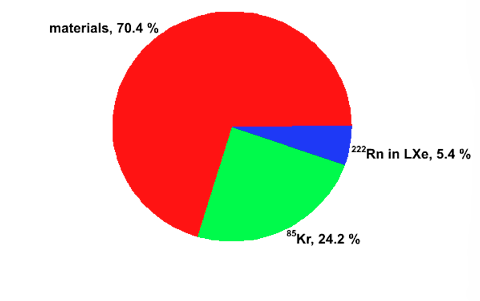
\includegraphics[height=0.3\linewidth]{plots/DataMC/pie_30kg_PassiveVeto.png}
\label{figPies_1}}
\subfigure[with veto coincidence cut]{
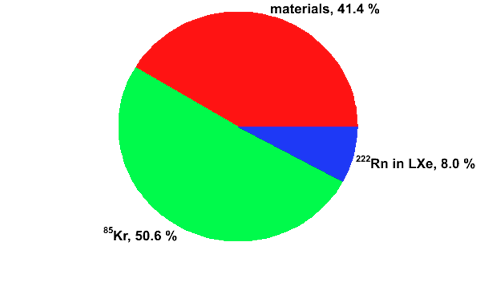
\includegraphics[height=0.3\linewidth]{plots/DataMC/pie_30kg_ActiveVeto.png}
\label{figPies_2}}
\caption[Contribution from various sources to the total background in the 30~kg fiducial volume]{Contribution from various sources to the total background in the 30~kg fiducial volume, without veto cut (a), and with the veto coincidence cut with an average energy threshold of 100~keV (b). The $^{\mathrm{nat}}$Kr concentration of 120~ppt measured in run07 has been assumed.}
\label{figPies}
\end{figure}


